\chapter{Konzept}
\label{ch:chapter04}
In diesem Kapitel wird darauf eingegangen, wie vorgegangen wurde, um verschiedene Konzepte zu entwickeln.
Dabei werden die vorher erwähnten Befragungen (\ref{ch:Recherche}) verwendet, um eine Lösung für die individuellen Probleme zu entwickeln.
Zudem wird der Stand der Technik betrachtet und ein Vergleich mit den Datenbankstrukturen gezogen.
Dies wird getan, da diese eine ähnliche Struktur wie die Profile und Berechtigungen. \textbf{\textcolor[rgb]{1,0,0}{Dies ist für mich kein verständlicher Satz.}}
Anschließend werden die Probleme aus den Befragungen quantifiziert, um daraus dann die verschiedenen Konzepte zu entwickeln.


\section{Konzeptentwicklung}
\label{sec:chapter04:Konzeptentwicklung}

\subsection{Stand der Technik}
\label{sec:chapter04:Stand}
In der Welt von Cloud Computing wird \ac{IAM} als Sicherheitsmaßnahme verwendet.
Dabei wird mittels \ac{IAM} die Identität und der Zugriff reguliert.
\ac{IAM} kann daher in die folgende fünf Punkte gegliedert werden.
\newline
\newline
1. Authentifizierung der Person
\newline
Dabei wird überprüft, ob die Person auch wirklich die ist, als welche diese sich ausgibt.
Um dies sicherzustellen, gibt es verschiedene Methoden.
Ein Nutzername mit einem Passwort ist die gängigste Methode, um dies zu tun. Dies wird von den meisten Webseiten und Computern verwendet.
Um die Authentifizierung sicherer zu gestalten, werden mehrere Faktoren berücksichtigt, um eine Person zu identifizieren.
Dies kann zum Beispiel durch einen Fingerabdruck stattfinden. \cite{IamIEEE} (S.1482)
\newline
\newline
2. Berechtigungsvergabe
\newline
Die Berechtigungsvergabe beschäftigt sich damit, welche Berechtigungen jeder Nutzer bekommt.
Dies wird mittels Autorisierungsrichtlinien gesichert, damit die Nutzer nur Zugriff auf die Ressourcen und Dienste haben, welche diese benötigen.
Dies wird mit Hilfe von Profilen erreicht, welche von der Organisation zugewiesen werden. \cite{IamIEEE} (S.1482)
\newline
\newline
3. Identitätsvergabe
\newline
Die Identitätsvergabe sorgt dafür, dass der Nutzer eine digitale ID oder Account erhält.
Wenn ein Mitarbeiter bei einem Unternehmen arbeitet, erhält dieser eine digitale Identität, um auf die Ressourcen des Unternehmens zugreifen zu können.
Dabei ist auch wichtig, dass der Mitarbeiter diese digitale Identität wieder verliert, wenn dieser das Unternehmen verlässt oder an einer anderen Stelle im Unternehmen arbeitet und nicht mehr seine alte digitale Identität benötigt.
\newline
\newline
4. Föderierte Identität
\newline
Dabei handelt es sich darum, dass die digitalen Identitäten über verschiedene Anwendungen und Organisationen gültig sind.
Dadurch werden die Informationen der digitalen Identität gespeichert.
Dies hat den Vorteil, dass der Nutzer sich nur einmal anmelden muss, um auf sämtliche seiner Ressourcen zugreifen zu können.
Dabei werden Protokolle wie SAML, OAuth oder OpenID verwendet.
Die Folge dadurch ist, dass der Nutzer sich nicht mehrere Passwörter sowie Accounts merken muss. \cite{IamIEEE} (S.1482)
\newline
\newline
5. Compliance Verwaltung
\newline
Die Compliance Verwaltung überprüft die Authentifizierung- und Zugriffaufzeichnungen, um sicher zu stellen, dass die Richtlinien und Sicherheitsstandards eingehalten wurden.
Diese Überprüfung ist notwendig für effektive Zugriffsregeln.
Zudem werden diese für Audits benötigt. \cite{IamIEEE} (S.1482)
\newline
\newline
\begin{figure}[h!]
 \centering
 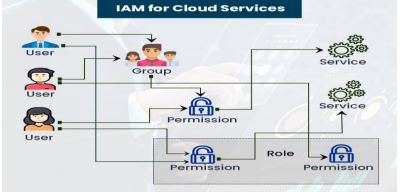
\includegraphics[width=1\textwidth]{gfx/Picture/IAMISH.PNG}
 \caption{IAM für Cloud Dienste \cite{Moha19} (Seite 3)}
 \label{fig:IMAISH}
\end{figure}
Dies ist ein Beispiel, wie die oben genannten Punkte umgesetzt werden können.
Dabei haben die Accounts der Personen entweder direkte Berechtigung oder diese werden mittels Gruppen verteilt.
Sobald der Account die Berechtigung hat, kann dieser auf die dahinter steckende Ressource zugreifen.
Die Berechtigungen können dabei auch mittels Profile zusammengefasst werden.
\newline
Dabei kann dies auf verschiedenen Wegen umgesetzt werden, da dieselbe Lösung für gewisse Fälle nicht funktioniert.
Zum Beispiel die Quelle \cite{Cal17}(S.208) beschreibt das Problem, wie die United States of America am besten mit ihren Verbündeten kooperieren soll.
Da es sich dabei um sensitive Informationen handelt, welche an verschiedene Partner vermittelt werden, muss der Zugriff reguliert werden.
Auch haben die verschiedenen Länder unterschiedliche Gesetzte, worauf geachtet werden muss. 
Deswegen gibt es nicht die eine Lösung, um eine solche Herausforderung zu lösen. \cite{Cal17} (S.208)


\subsection{Vergleich mit Datenbanken}
\label{sec:chapter04:DB}
Die Helvetia verwendet zum Speichern der Informationen für die Berechtigungsstruktur sogenannte HV-Tabellen.
Bei diesen HV-Tabellen handelt es sich, um DB2-Tabellen.
Zudem besteht eine Ähnlichkeit zwischen dem Nutzer und Profil in der Berechtigungsstruktur zu dem Account und Gruppe in Datenbanken. \textbf{\textcolor[rgb]{1,0,0}{Der Satz ist für mich so nicht verständlich.}}
Deswegen wird betrachtet, wie der Standard von Accounts und Gruppen innerhalb von Datenbanken ist.
\newline
Berechtigungen für Rollen werden mittels GRANT...ON...TO...[GRANT OPTION] vergeben.
Dabei wird für die spezifische Berechtigung, zum Beispiel eine View und Account oder Gruppen angegeben.
Zudem kann auch hinzugefügt werden, ob die Rolle die Berechtigung hat, anderen Accounts die Berechtigungen zu geben.\cite{Ram09} (S.474-475)
\newline
Wenn man sich zum Beispiel das Bild (\ref{fig:Berch}) ansieht, könnte zum Beispiel der Befehl wie folgt aussehen:
\newline
\newline
GRANT UPDATE ON PKU00 TO L895.
\newline
\newline
Das würde in diesem Beispiel bedeuten, dass der Nutzer L895 die Bearbeitungsberechtigung für die Ressource PKU00 erhalten hat.
Dabei kommt auch die Frage, was man eher verwenden sollte.
Individuelle Berechtigungsvergabe oder Gruppenvergabe für die Accounts.
Microsoft hat folgendes als Best Practice definiert:
\newline
\newline
\textit{"`To simplify administration, create groups and assign each group permission to functional areas and model objects.
You can then add and remove users from the groups without accessing the Master Data Manager UI.
\newline
\newline
Do not assign additional permissions to an individual user, and do not include a user in multiple groups that have access to Master Data Manager. In addition, do not use hierarchy member permissions unless you want a group to have limited access to specific members."'} \cite{Micro}
\newline
\newline
Microsoft gibt an, dass man Gruppen erstellen, die individuellen Nutzer keine zusätzlichen Berechtigungen bekommen sollen und nicht in mehreren Gruppen sein soll, die Zugriff auf den Master Data Manager haben. \textbf{\textcolor[rgb]{1,0,0}{Dies ist für mich kein verständlicher Satz.}}
Und auch IBM gibt in seiner Best Practice an, dass Angestellte in einem Unternehmen mittels Gruppen organisiert werden sollten. \cite{IBMGroup}

\section{Herausforderung und Anforderungen}
\label{sec:chapter04:Herausforderung}
Bei der Recherche (\ref{ch:Recherche}) sind verschiedene Herausforderungen und Anforderungen aufgetreten.
Um qualitativ ein Konzept entwickeln zu können, müssen diese Herausforderungen und Anforderungen aufgelistet und analysiert werden.
\begin{itemize}
	\item Performance der Tabellen erhöhen (effizientere Verifizierung der Mitarbeiter)
	\item Übersichtlicher gestalten
	\item Rekursive Beziehungen verhindern
	\item Hierarchie verringern
	\item \ac{K/W}
\end{itemize}
Um diese zu quantifizieren zu können, wird eine Prioritätsanalyse (\ref{fig:Prio}) verwendet, um festzustellen, wie die Priorität für die Konzepte sein muss. \cite{BdIufH}
Bei der Prioritätsanalyse wurde sich für ein vier Punktesystem entschieden.
\newline
Im Vergleich zwischen der Performance und der Übersichtlichkeit, wurden Performance drei Punkte gegeben und die Übersichtlichkeit hat nur einen Punkt erhalten, da die Performance eine der Grundanforderungen ist, weswegen die Berechtigungsstruktur geändert werden soll.
Die Übersichtlichkeit dazu ist weniger wichtig.
Die Performance und die Rekursion haben jeweils zwei Punkte bekommen, da eine performante Struktur keine rekursiven Beziehungen enthält.
Die Performance hat vier Punkte zur Hierarchie und die Hierarchie zur Performance null Punkten erhalten, weil die Verringerung der Hierarchie kaum einen Einfluss auf die jährliche Rezertifizierung hat. 
\ac{K/W} sowie Performance haben jeweils zwei Punkte bekommen.
Dies liegt daran, dass neben der Performance die \ac{K/W} elementar sind, da eine Struktur, die sich kaum warten lässt, mehr Ressourcen in der Zukunft kosten wird.
Zwischen der Übersichtlichkeit und der Rekursion wurden der Rekursion drei Punkte gegeben und der Übersichtlichkeit nur einen, weil rekursive Strukturen unübersichtlicher sind und es daher wichtiger ist, dass es keine gibt.
Übersichtlichkeit und Hierarchie haben beide zwei Punkte erhalten, da beide eine gleiche Rolle bei der Lesbarkeit der Struktur spielen.
Übersichtlichkeit, sowie Rekursion und Hierarchie bekommen einen Punkt im Vergleich zu \ac{K/W}, weil dieser Punkt langfristig eine wichtige Rolle spielt, und die anderen drei Punkte sollten keine Probleme sein, sofern sich an die Konventionen gehalten wird, damit die Struktur wartbar bleibt.
Die Rekursion bekommt zur Hierarchie vier Punkte und die Hierarchie zur Rekursion null Punkte, da eine rekursive Beziehung die Hierarchie automatisch unendlich macht.
\newline
\newline
Wenn man dies auswertet, bekommt die Performance einen Gewichtsfaktor von 27,5\%, die Übersichtlichkeit 12,5\%, die Rekursion 25\%, die Hierarchie 7,5\% und \ac{K/W} 27,5\%.
Dadurch sieht die Rangfolge wie folgt aus:
\begin{enumerate}
	\item Performance | \ac{K/W}
	\item Rekursion
	\item Übersichtlichkeit
	\item Hierarchie
\end{enumerate}
Anhand dieser Reihenfolge werden die folgenden Konzepte entwickelt.
\begin{figure}[h!]
 \centering
 \includegraphics[width=1\textwidth]{gfx/Picture/Prioritatätsanalyse.PNG}
 \caption{Prioritätsanalyse der Kriterien}
 \label{fig:Prio}
\end{figure}

\section{Konzept hierarchische Struktur}
\label{sec:chapter04:Struktur}
Das erste Konzept für die Struktur ist wie folgt aufgebaut.
\begin{figure}[h!]
 \centering
 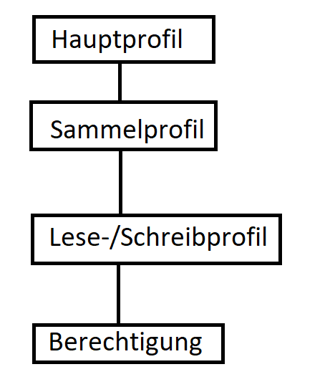
\includegraphics[width=0.75\textwidth]{gfx/Picture/Hierarchie.PNG}
 \caption{Hierarchie für Konzept Struktur}
 \label{fig:Struktur}
\end{figure}
Wie man in der Graphik (\ref{fig:Teil}) erkennen kann, gibt es bei der aktuellen Berechtigungsstruktur keine Struktur.
Um dementsprechend die genannten Problem zu beheben, wurde die neue Struktur (\ref{fig:Struktur}) entwickelt.
Um die \ac{K/W} zu verbessern, wurden die folgenden Konventionen für dieses Konzept entwickelt.
Anzumerken dabei ist, dass es trotzdem ein Aufwand ist, diese durchzusetzen und zu implementieren.
\textbf{\textcolor[rgb]{1,0,0}{Das Folgende ist für mich eine Aufzählung }}
Profile enthalten nur noch Profile oder Berechtigungen.
Die Berechtigungsstruktur soll nur noch eine Hierarchietiefe von maximal vier haben.
Die erste Hierarchiestufe enthält das Standardprofil, welche dem Nutzer gegeben wird.
Die zweite Hierarchiestufe enthält die jeweiligen Sammellese- und -schreibprofile, die jeweils in die Fachbereiche getrennt sind.
Die dritte Hierarchiestufe enthält die individuellen Lese- und Schreibprofile.
Die vierte Stufe enthält die Berechtigungen.
Manche der bestehenden Profile beinhalten aktuell, was zukünftig Hauptprofile wären.
In solchen Fällen würden diese Profile zu Hauptprofilen werden und vom vorherigen Hauptprofil separiert werden.
Manche Fachbereiche haben aufzählende Profile (\ref{fig:Profile}).
Diese Profile sollen nur noch über die Berechtigungen für den eigenen Vorgang enthalten, sodass ein Privas Profil nur Privas Berechtigungen enthält.
Die Berechtigung die verloren gehen würden eigene Profile bekommen und würden über ein anderes Sammelprofil dem Hauptprofil hinzugefügt werden.
Sollte ein Nutzer weitere Berechtigungen benötigen, würden diese über ein anderes Hauptprofil, welches am ehesten für die Aufgabe passt, zugeordnet.
Wenn ein Account reaktiviert wird, muss dieser rezertifiziert werden.
\newline
Diese Konventionen sollen verhindern, dass die Struktur weiter wächst und das man ohne Probleme feststellen kann, was für Berechtigungen ein Profil hat.
Zudem hat es den Vorteil, dass rekursive Beziehungen, sowie redundante Berechtigungsvergabe nicht möglich sind, da die Profile nur noch Profile oder Berechtigungen enthalten, die nicht mehr auf sich gegenseitig zeigen.
Dadurch soll auch die Übersichtlichkeit verbessert und das Hierarchieproblem auf ein Minimum gebracht werden.
Außerdem sollte die Performance verbessert werden. Dies durch die fehlenden rekursiven Beziehungen, sowie die Vereinfachung der Struktur, mit der Reduktion der Berechtigungen.
\begin{figure}[h!]
\hspace*{-2cm}
 \centering
 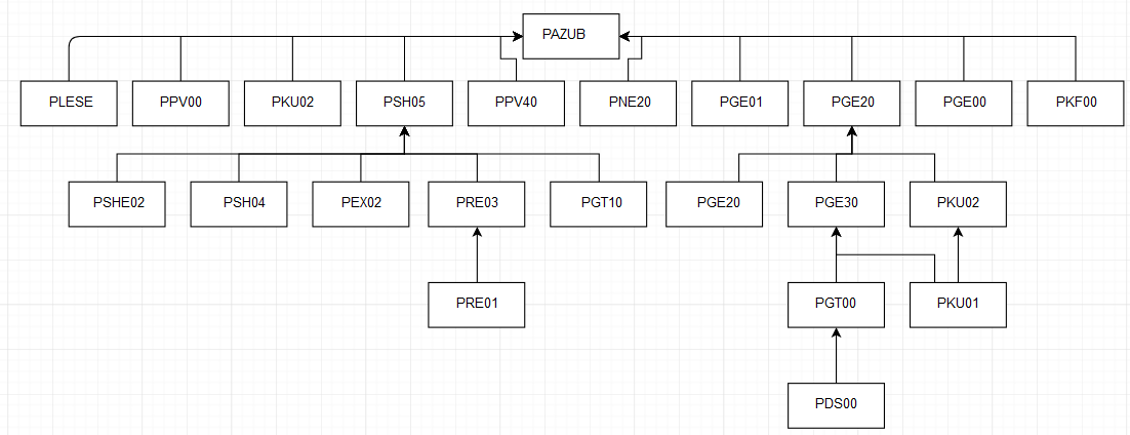
\includegraphics[width=1.25\textwidth]{gfx/Picture/Vorher.PNG}
 \caption{Beispiel der bestehenden Berechtigungsstruktur}
 \label{fig:AltBer}
\hspace*{-2cm}
 \centering
 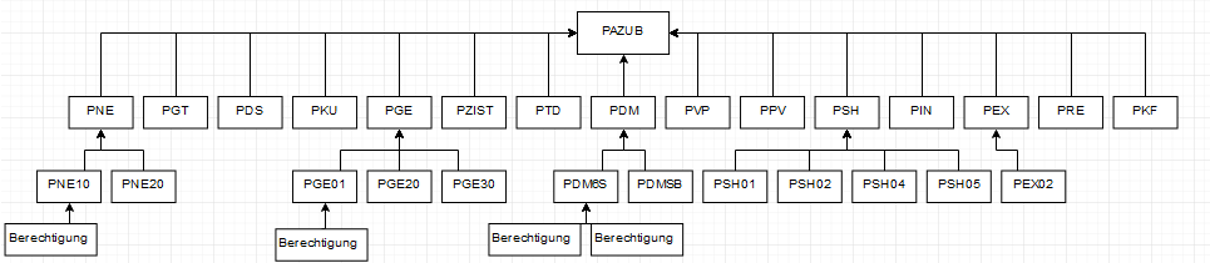
\includegraphics[width=1.25\textwidth]{gfx/Picture/Nachher.PNG}
 \caption{Beispiel der neuen Berechtigungsstruktur}
 \label{fig:NeuBer}
\end{figure}
\newpage
Das Bild (\ref{fig:AltBer}) zeigt eine bestehende Berechtigungsstruktur.
(\ref{fig:AltBer}) hingegen bildet die Struktur nach den neuen Konventionen dar.
Diese beide Bilder wurden den IT-Spezialisten gezeigt, die befragt wurden.
Einheitlich haben alle befragten IT-Spezialisten angegeben, dass Sie die neue Struktur übersichtlicher finden und diese einfacher zu verstehen ist.
Zudem kann auch erkannt werden, dass die Hierarchie verringert wurde.
\newline
Das aktuelle Verfahren, das verwendet wird, um die Berechtigung zu überprüfen, gleicht einem Insertion-Sort.
Dabei wird jedes einzelne Profil durchgegangen, bis die gewünschte Berechtigung gefunden wurde.
Dies weißt eine Komplexität von n im Optimalfall und $n^2$ im schlimmsten Falle auf.
n beschreibt dabei, die Anzahl von Profilen/Berechtigungen, die der Algorithmus durchlaufen muss. \cite{weblogIn,log} (S. 12)
\newline
Bei der neuen Struktur kann ein Merge-Sort genutzt werden.
Dabei achtet der Algorithmus auf bestimmte Eigenschaften der Profile.
Würde zum Beispiel verlangt werden, dass der Nutzer eine Berechtigung für PNE10 hat, würde nur der Baum von PNE durchsucht werden und in diesem Falle direkt PNE10 ausgewählt werden.
Dieser Suchalgorithmus ist komplexer als der Insertion-Sort. Er ist jedoch deutlich effizienter bei einer größeren Menge von Profilen und Berechtigungen.
Die Komplexität beläuft bei ihm auf n*log(n) im besten, wie auch im schlechtesten Fall. \cite{weblogMer,log} (S. 12)
\newline
Wenn beispielsweise n = $100$ wäre, würden die Ergebnisse wie folgt aussehen:
\newline
\newline
Best-Case(Insert) = $100$
\newline
Worst-Case(Insert) = $100^2 = 10.000$
\newline
\newline
Best-Case(Merge) = $100*log(100) = 200$
\newline
Worst-Case(Merge) = $100*log(100) = 200$
\newline
\newline
Wie man erkennen kann, ist der neue Algorithmus im Best-Case langsamer, aber im Worst-Case deutlich schneller und bietet allgemeinen eine konsistente Zeit, welche für eine Versicherung wichtig ist.
Der Insertion-Sort sowie der Merge-Sort haben auch eine average Formel: \cite{weblogMer,weblogIn}
\newline
\newline
Average(Insert) = $100^2 = 10.000$
\newline
\newline
Average(Merge) = $100*log(100) = 200$
\newline
\newline
Man kann erkennen, dass im normalen Falle die neue Struktur mit dem Merge-Sort deutlich effektiver ist als die bestehende Struktur.
Diese würde durchschnittlich $50$ mal effektiver sein.
\newpage
\section{Konzept Minimalistisch}
\label{sec:chapter04:minimal}
Im Gespräch der IT-Spezialisten kam der Vorschlag auf, dass man einen minimalistischen Ansatz nutzen könnte.
Dabei haben die IT-Spezialisten folgende Vorschläge für die Konventionen gemacht:
\newline
Profile enthalten nur noch Profile oder Berechtigungen.
Es werden Standardprofile für die jeweiligen Abteilungen entwickelt.
Zusätzliche Berechtigungen werden dem Nutzer direkt zu geordnet.
Wenn ein Account reaktiviert wird, muss dieser rezertifiziert werden.
\begin{figure}[h!]
 \centering
 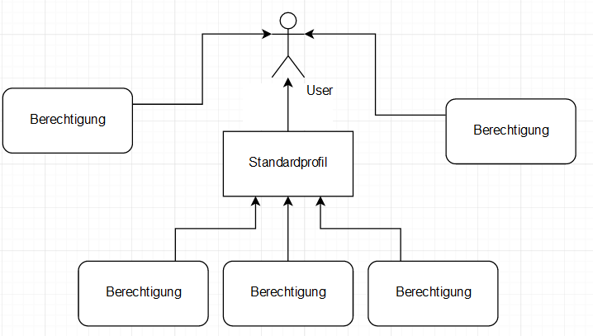
\includegraphics[width=1\textwidth]{gfx/Picture/Minimal.PNG}
 \caption{Beispiel für das Konzept Minimalistisch}
 \label{fig:Min}
\end{figure}
Die IT-Spezialisten fanden auch, dass dies übersichtlicher als die bestehende Struktur ist.
Dieses Konzept hat den Vorteil, dass es kaum noch eine Hierarchie gibt.
Dadurch entfällt das Problem der Rekursion sowie redundante Berechtigungsvergabe.
Die \ac{K/W} ist einfacher in diesem Sinne, da nur überprüft werden muss, ob die Standardprofile über die notwendigen Berechtigungen verfügen.
Auf der anderen Seite ist die Entwicklung aufwendig, da ersteinmal bestimmt werden muss, welche Berechtigungen für einen Fachbereich notwendig sind. Ebenso muss sichergestellt werden, dass alle Nutzer ihre Berechtigungen beibehalten.
Es besteht nämlich die Gefahr, dass bei dem Wechsel Berechtigungen verloren gehen.
\newline
\newline
Wenn man (\ref{fig:Min}) betrachtet, kann für diese Struktur nur ein Insertion-Sort verwendet werden.
Dies liegt daran, dass der Sort die individuellen Einträge durchlesen muss, da es keine Information gibt, wo welche Berechtigung ist.
Die aktuelle Struktur verwendet auch einen Insertion-Sort, aufgrund des gleichen Problems.
Jedoch ist zu bemerken, dass die Anzahl der n bei diesem Konzept geringer ist, da es nicht die verschiedenen Profile mit Redundanzen gibt.
\newline
\newline
Ein Hauptprofil hatte zum Beispiel $110$ Profile mit enthalten Berechtigungen.
Von diesen $110$ waren $78$ redundante Profile.
Da Profile eine Ansammlung von Berechtigungen sind, ist die Anzahl von redundanten Berechtigungen deutlich höher.
Wenn man nur den Unterschied zwischen der bestehenden Struktur mit der minimalistischen Struktur macht, erhält man folgenden Vergleich:
\newline
\newline
Best-Case(Alte Struktur) = $110$
\newline
Worst-Case(Insert) = $110^2 = 12.100$
\newline
Average(Insert) = $110^2 = 12.100$
\newline
\newline
Best-Case(Neue Struktur) = $32$
\newline
Worst-Case(Neue Struktur) = $32^2 = 1.024$
\newline
Average(Neue Struktur) = $32^2 = 1.024$
\newline
\newline
Man kann feststellen, dass obwohl die neue Struktur nicht über einen effizienteren Algorithmus verfügt, dieser trotzdem eine bessere Performance hat.
Die neue Struktur wäre in diesem Beispiel ca. $12$ mal performanter als die bestehende Struktur.